%% SW arkitektur: Fejlhåndtering

Systemet kan håndterer fejl og disse vil blive gemt i en fejllog som bliver gemt på Master. 

Fejlhåndteringen bliver klaret af en klasse på Devkit8000 som håndterer at skrive det rigtige fejl ud i en \verb+.txt+-fil. Klassen vil blive kaldt med en fejlkode hver gang fejl opstår. Klassen forstår så at skrive den rigtige fejl ind i txt filen ud fra den pågældende fejlkode den har modtaget som attribut. 

Alle funktioner vil returnere et negativt heltal som repræsenterer en fejlkoden som klassen kan tolke på.

\begin{figure}[htbp] \centering
{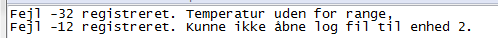
\includegraphics[scale=0.7]{filer/pics/Errortxt}}
\caption{udsnit af Error log}
\label{fig:ErrorLog}
\end{figure}

Billedet på figur \ref{fig:ErrorLog} viser hvordan 2 fejl i error-loggen kunne se ud.